\documentclass[twocolumn,times]{aastex701}

\usepackage{graphicx}
\usepackage{amsmath,amssymb}
\usepackage{booktabs}
\usepackage{xcolor}
\usepackage{tikz}
\usetikzlibrary{arrows.meta,positioning}

\graphicspath{{assets/}}

\newcommand{\AuroraLF}{AuroraLF}
\newcommand{\Msun}{M_\odot}
\newcommand{\Muv}{M_{\rm UV}}
\newcommand{\Mh}{M_{\rm h}}
\newcommand{\SFR}{\mathrm{SFR}}
\newcommand{\Zsun}{Z_\odot}
\newcommand{\dd}{\mathrm{d}}

\shorttitle{AuroraLF Pop III UVLF Diagnostics}
\shortauthors{AuroraLF Project Team}

\begin{document}

\title{\AuroraLF: time-resolved high-redshift ultraviolet luminosity functions with Population III diagnostics}

\author{AuroraLF Project Team}
\affiliation{AuroraLF project}
\email{auroralf-project@example.org}

\begin{abstract}
\AuroraLF\ is a Monte Carlo framework for modelling the ultraviolet luminosity function (UVLF) of high-redshift galaxies. The present project stage uses a Population II baseline as the reference calculation, connecting halo assembly histories, delayed star formation, diagnostic gas metallicities, stellar-population synthesis and halo-mass-function weighting in a single reproducible workflow. The main current extension is a Population III minihalo channel. This draft summarizes the model framework, the present diagnostic results, and the completed Population III pair-instability supernova (PISN) rate calculation. The PISN calculation converts the Population III star-formation-rate density into an intrinsic comoving rate density and shows how the result depends on the upper halo-mass boundary of the Population III channel.
\end{abstract}

\keywords{High-redshift galaxies --- Luminosity function --- Population III stars --- Pair-instability supernovae --- Galaxy formation}

\section{Introduction}\label{sec:introduction}

High-redshift UV luminosity functions measured in the JWST era require models that retain explicit time information. A single relation between halo mass and UV luminosity cannot capture rapid halo growth, delayed star formation, bursty scatter or residual Population III contributions. The purpose of \AuroraLF\ is therefore not to fit an analytic luminosity--mass mapping directly. Instead, each halo growth history is propagated into a star-formation history, a metallicity diagnostic and a UV luminosity, and the resulting luminosity distribution is integrated over the halo mass function.

The current framework has two scientific roles. First, it defines a Population II baseline using McBride-style Monte Carlo halo assembly histories \citep{McBride2009}, a Reed07 halo mass function \citep{Reed2007} and BPASS-based Population II stellar-population synthesis \citep{Eldridge2017,Stanway2018}. Second, and most importantly for the present stage, it introduces a Population III minihalo channel in the same time-resolved framework. This channel is intended to test whether early, metal-free star formation can provide an observable contribution to high-redshift UV emission and to independent transient-rate diagnostics. Population II top-heavy IMF variants are retained only as optional historical comparisons and are not treated as the main interpretation in this draft.

\section{Model framework}\label{sec:model}

\subsection{Time-resolved halo assembly histories}\label{subsec:mah}

For a halo observed at final mass $M_0$ and redshift $z_0$, the reference halo-assembly backend draws the Appendix A parameters $(\beta,\gamma)$ of \citet{McBride2009} by rejection sampling from their mass-dependent mixture distribution. A small power-law component is sampled with $\gamma=0$, while the dominant joint component samples $(\beta,y')$ and maps $y'$ to $\gamma$. Each accepted pair defines
\begin{equation}
  M_{\rm h}(z)
  =
  M_0
  \left(\frac{1+z}{1+z_0}\right)^\beta
  \exp[-\gamma(z-z_0)] .
  \label{eq:mcbride-mah}
\end{equation}
The halo accretion rate used by the star-formation calculation is obtained by differentiating this history with respect to cosmic time,
\begin{equation}
  \dot{M}_{\rm h}(z)
  =
  -H(z)(1+z)M_{\rm h}(z)
  \left[\frac{\beta}{1+z}-\gamma\right].
  \label{eq:mcbride-mdot}
\end{equation}
The Monte Carlo ensemble is therefore the collection of accepted McBride histories on the adopted redshift grid, truncated below the adopted mass floor. The derivative is evaluated on the time grid and converted to $\mathrm{M}_\odot\,\mathrm{yr}^{-1}$ when inserted into the SFR equations below. Figure~\ref{fig:mcbride-mah} illustrates a 1000-draw McB09 parameter sample and compares the resulting high-redshift MAH shapes with THESAN-dark-1 LHaloTree histories at $z_f=10.98$ \citep{Kannan2022}. This comparison is used as a shape-level validation beyond the redshift range calibrated in \citet{McBride2009}, rather than as a one-to-one calibration of individual merger histories. For the mass bin shown, the THESAN median remains inside the McB09 16--84 percentile envelope at all stored snapshots, and the median offset is at most $0.13$ dex over the last $100$ Myr before the final snapshot. The offset reaches $0.51$ dex at the earliest stored times, where the THESAN median lies below the McB09 median, so the agreement should be described as consistency within the intrinsic halo-to-halo scatter. The present draft therefore uses the unified semi-analytic McBride baseline as the reference calculation, while retaining simulation-backed histories as validation backends.

\begin{figure*}[tbp!]
\centering
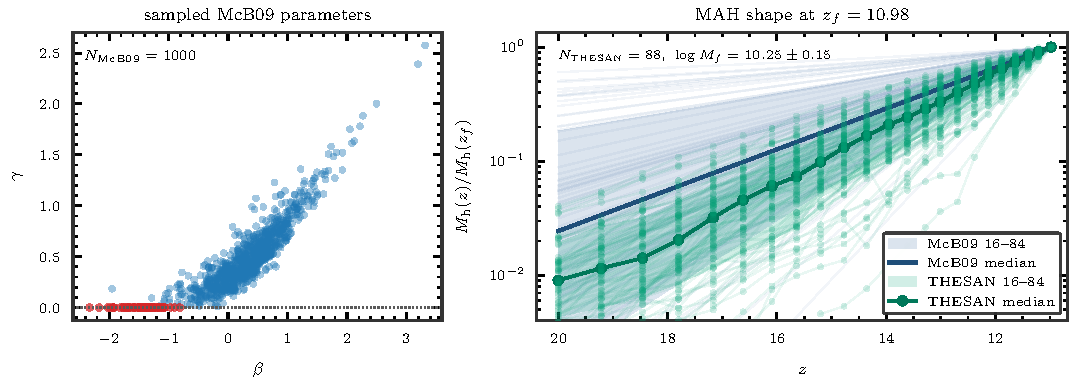
\includegraphics[width=\textwidth]{mcbride_mah_sampling_illustration.pdf}
\caption{McBride-style halo assembly sampling and high-redshift validation used by the reference MAH backend. Left: 1000 accepted Appendix A draws in the $(\beta,\gamma)$ plane; red points mark the $\gamma=0$ power-law component and blue points mark the joint component. Right: normalized halo assembly histories generated by Equation~(\ref{eq:mcbride-mah}) are compared with THESAN-dark-1 LHaloTree histories. The THESAN sample selects $N=88$ halos with $\log_{10}(M_f/M_\odot)=10.25\pm0.15$ at $z_f=10.98$. Blue shows the McB09 16--84 percentile envelope and median computed from the same 1000 draws; green shows the corresponding THESAN envelope, median and raw snapshot points. The comparison is normalized by each halo's final mass, so it tests MAH shape rather than the final halo-mass distribution, and is used here as a percentile-band consistency check.}
\label{fig:mcbride-mah}
\end{figure*}

\subsection{Stellar-population assignment and the Pop III-to-Pop II transition}\label{subsec:population-routing}

The separation between Population III and Population II star formation is defined at the source-time level, prior to the SFR and UV calculations. The Population II branch is activated once the halo reaches the atomic-cooling threshold, $T_{\rm vir}=10^4\,{\rm K}$ with $\mu=0.61$ \citep[e.g.][]{BarkanaLoeb2001}. Below this boundary, the Population III branch corresponds to the minihalo interval between the LW-regulated molecular-cooling floor and an upper mass scale $M_{\rm up}^{\rm III}$, which is set to the atomic-cooling mass in the fiducial calculation. The molecular-cooling floor follows the LW-feedback scaling used in Population III minihalo models \citep{Machacek2001,Venditti2023},
\begin{equation}
  M_{\rm min,III}(z,J_{21})
  = 3.3\times 10^7\,(1+z)^{-3/2}
    \bigl[1+2J_{21}^{0.6}\bigr]\,M_\odot .
\end{equation}
Figure~\ref{fig:cooling-window} shows the resulting mass routing for the zero-external-LW case used as the fiducial reference.

\begin{figure*}[tbp!]
\centering
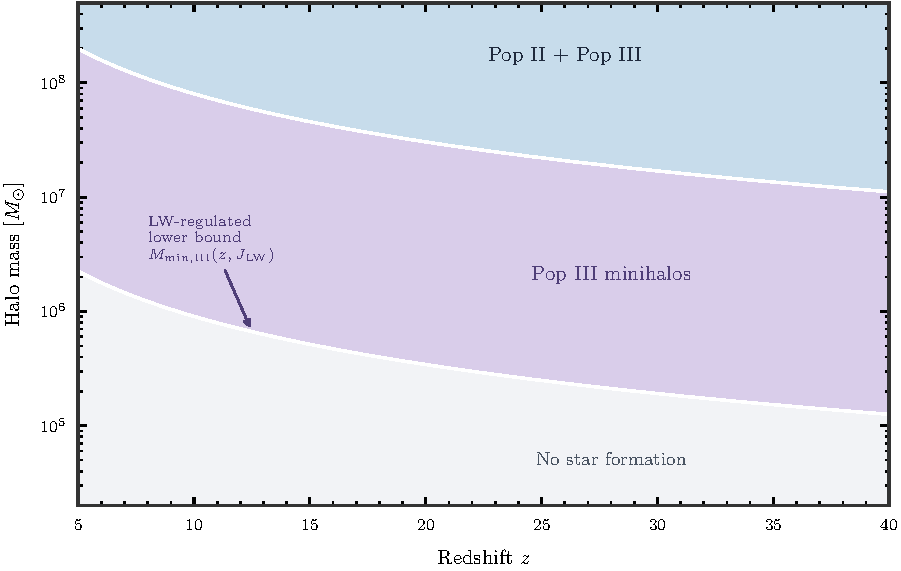
\includegraphics[width=0.75\textwidth]{cooling_mass_regions.pdf}
\caption{Cooling-based mass routing used by the Population III extension. The lower boundary is the LW-regulated molecular-cooling floor $M_{\rm min,III}(z,J_{\rm LW})$. Halos below this floor do not form stars in this channel, minihalos between the molecular and atomic-cooling boundaries are assigned to Population III star formation, and halos above the atomic-cooling boundary enter the Population II-dominated channel. The blue atomic-cooling region can also be used for explicit fixed-$M_{\rm up}^{\rm III}$ Population III sensitivity tests, but this is not the fiducial routing.}
\label{fig:cooling-window}
\end{figure*}

Operationally, this assignment should be interpreted as a cooling-based routing prescription rather than a closed chemical-enrichment transition. The current Population III SFR is weighted by
\begin{equation}
  f_{\rm duty}^{\rm III}
  = \exp[-M_{\rm min,III}/M_{\rm h}]\,
    \exp[-M_{\rm h}/M_{\rm up}^{\rm III}],
\end{equation}
and the corresponding source term is
\begin{equation}
  \dot M_\star^{\rm III}
  =
  f_{\rm b}\,f_\star^{\rm III}(M_{\rm h})\,
  f_{\rm duty}^{\rm III}(M_{\rm h},z)\,
  \dot{M}_{\rm h} .
\end{equation}
The fiducial parameters are $\epsilon_\star^{\rm III}=10^{-3}$ and $M_p^{\rm III}=10^7\,M_\odot$. Population III enrichment is not yet propagated back into the Population II metallicity calculation. The fixed $M_{\rm up}^{\rm III}=10^{10}\,M_\odot$ option used later in the PISN comparison therefore serves as a sensitivity test of the allowed Population III halo interval, rather than a modification to the fiducial transition rule.

\subsection{Population II star formation and metallicity}\label{subsec:popii}

Given this assignment, the instantaneous Population II star-formation source term is written along each halo assembly history using the halo-accretion-based form adopted in high-redshift luminosity-function and 21 cm modelling \citep{Sun2016,Mirocha2017},
\begin{equation}
  \mathrm{SFR}(t) = f_{\rm b}\, f_\star(M_{\rm h})\,\dot{M}_{\rm h},
\end{equation}
where $\dot{M}_{\rm h}$ is expressed in $\mathrm{M}_\odot\,\mathrm{yr}^{-1}$. The production UVLF calculation follows the extended-burst delay kernel adopted by \citet{Yue2016}, which is based on a dynamical timescale,
\begin{equation}
  g(t-t') \propto (t-t')\exp[-(t-t')/(\kappa t_{\rm d})],
\end{equation}
which convolves the source-time halo accretion term $f_\star(M_{\rm h})\dot{M}_{\rm h}$.

{\color{blue}
Metallicity is currently treated as a diagnostic along fixed halo and star-formation histories. The mass--metallicity relation option provides an empirical prior based on high-redshift FIRE-2 and JADES MZR fits \citep{Ma2016,Curti2024}, while the regulator option uses a simplified gas-regulator metallicity closure motivated by \citet{Lilly2013} and \citet{PengMaiolino2014}, computing a gas metallicity of the form
\begin{equation}
  Z_{\rm gas} = Z_0 +
  \frac{y}{1 + M_{\rm gas}/M_\star + \lambda_Z/(1-R)} .
\end{equation}
The quantities $Z_{\rm gas}$ and $Z_{\rm birth}$ do not feed back into the SFR in the present calculation. They are used to track early internal enrichment and to provide a reference point for later closure of Population III enrichment.
}

\subsection{UVLF estimation}\label{subsec:uvlf}

The stellar-population module convolves the SFR history with a stellar-population synthesis table to obtain the 1600 \AA\ UV luminosity. Population III UV tables are taken from the very metal-poor burst models of \citet{Raiter2010}. After the Population II and Population III source-time histories are assigned, the UVLF is estimated with a two-level Monte Carlo calculation,
\begin{equation}
  \phi(x,z) =
  \int \mathrm{d}\log_{10}M_{\rm h}\,
  \frac{\mathrm{d} n}{\mathrm{d}\log_{10}M_{\rm h}}(M_{\rm h},z)\,
  P(x\mid M_{\rm h},z),
\end{equation}
where $x$ may denote either $M_{\rm UV}$ or UV luminosity. The outer sampling is performed in $\log_{10}M_{\rm h}$, and the Reed07 halo mass function \citep{Reed2007} is converted according to
\begin{equation}
  \frac{\mathrm{d} n}{\mathrm{d}\log_{10}M_{\rm h}}
  = M_{\rm h}\ln 10\,\frac{\mathrm{d} n}{\mathrm{d}M_{\rm h}}.
\end{equation}
For each final halo mass, multiple halo histories and luminosity realizations are generated. The halo-mass-function weight of a mass bin is distributed over its internal luminosity realizations. The upper halo-mass mode and the LW background are retained as parameters for systematic scans, motivated by the sensitivity of Population III observability to the allowed halo-mass interval \citep{Visbal2015,Visbal2017}.

\begin{figure*}[tbp!]
\centering
\resizebox{\textwidth}{!}{%
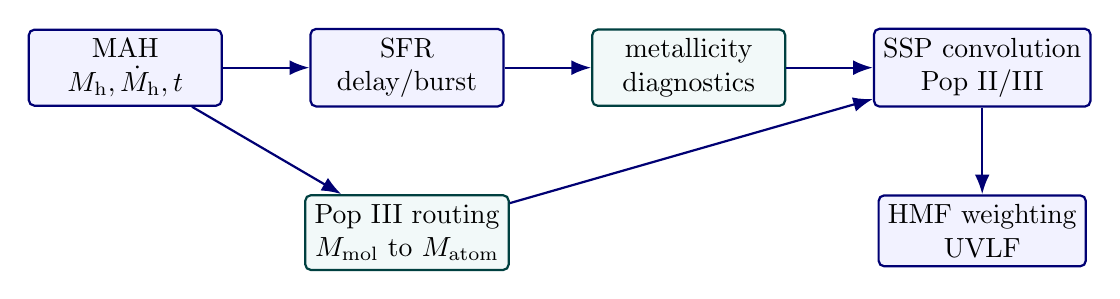
\begin{tikzpicture}[
  node distance=1.10cm,
  box/.style={draw=blue!45!black, rounded corners=2pt, thick, align=center,
    minimum width=2.45cm, minimum height=0.72cm, fill=blue!5},
  opt/.style={draw=teal!50!black, rounded corners=2pt, thick, align=center,
    minimum width=2.45cm, minimum height=0.72cm, fill=teal!5},
  flow/.style={-{Latex[length=2.5mm]}, thick, draw=blue!45!black}
]
\node[box] (mah) {MAH\\$M_{\rm h},\dot{M}_{\rm h},t$};
\node[box, right=of mah] (sfr) {SFR\\delay/burst};
\node[opt, right=of sfr] (metal) {metallicity\\diagnostics};
\node[box, right=of metal] (ssp) {SSP convolution\\Pop~II/III};
\node[box, below=of ssp] (uvlf) {HMF weighting\\UVLF};
\node[opt, below=of sfr] (popiii) {Pop~III routing\\$M_{\rm mol}$ to $M_{\rm atom}$};
\draw[flow] (mah) -- (sfr);
\draw[flow] (sfr) -- (metal);
\draw[flow] (metal) -- (ssp);
\draw[flow] (ssp) -- (uvlf);
\draw[flow] (mah) -- (popiii);
\draw[flow] (popiii) -- (ssp);
\end{tikzpicture}}
\caption{Numerical structure of the current \AuroraLF\ calculation. The Population II baseline is complete through halo assembly, SFR, metallicity diagnostics, stellar-population convolution and HMF weighting. The Population III channel is connected through mass routing, SFR and UV diagnostics, while feedback and enrichment have not yet been closed back into the Population II metallicity calculation.}
\label{fig:pipeline}
\end{figure*}

\section{Current results}\label{sec:results}

\begin{table*}[tbp!]
\caption{Quantitative results currently included in the manuscript.}
\label{tab:current-results}
\begin{tabular}{ll}
\toprule
\parbox[t]{0.25\textwidth}{Diagnostic} & \parbox[t]{0.66\textwidth}{Current result} \\
\midrule
\parbox[t]{0.25\textwidth}{Population II UVLF baseline} &
\parbox[t]{0.66\textwidth}{The canonical Population II model is calibrated at $z=6$, with a median model/observation offset of $-0.043$ dex across the adopted UVLF data. At $z=12.5$, the same baseline has a median offset of $-1.235$ dex, corresponding to a median model/observation ratio of $5.8\%$.} \\
\parbox[t]{0.25\textwidth}{Population III cooling window} &
\parbox[t]{0.66\textwidth}{For $J_{21}=0$, $M_{\rm min,III}/M_{\rm Jeans}=87.3$, 17.3 and 6.55 at $z=10$, 20 and 30. The corresponding $M_{\rm min,III}$ values are $5.91\times10^5$, $3.10\times10^5$ and $2.10\times10^5\,M_\odot$, below the atomic-cooling threshold.} \\
\parbox[t]{0.25\textwidth}{Regulator metallicity scale} &
\parbox[t]{0.66\textwidth}{At $\log M_{\rm h}=8.5$, the offset relative to the \citet{Ventura2024} polluted-IGM scale is $-0.60$ to $+0.13$ dex. At $\log M_{\rm h}=9.5$, it evolves from $-0.03$ dex at $z=7$ to $+3.62$ dex at $z=15$, where the massive-halo bin is statistically fragile.} \\
\bottomrule
\end{tabular}
\end{table*}

\subsection{Population II baseline at high redshift}\label{subsec:popii-baseline}

Figure~\ref{fig:popii-baseline-fit} compares the same canonical Population II baseline against UVLF data at $z=6$ and $z=12.5$. The $z=6$ comparison provides the low-redshift calibration check: across the plotted data sets the median model/observation offset is $-0.043$ dex, with a mean absolute offset of $0.148$ dex. The same model under-produces the $z=12.5$ UVLF, where the median offset is $-1.235$ dex and the median model/observation ratio is $5.8\%$. This establishes a clear reference for the Population III extension: if the Population II baseline is held fixed, the high-redshift bright end remains under-produced. The next comparison should therefore quantify the contribution from Population III minihalos and their short-lived UV output before treating any Population II top-heavy IMF variant as a default explanation.

\begin{figure*}[tbp!]
\centering
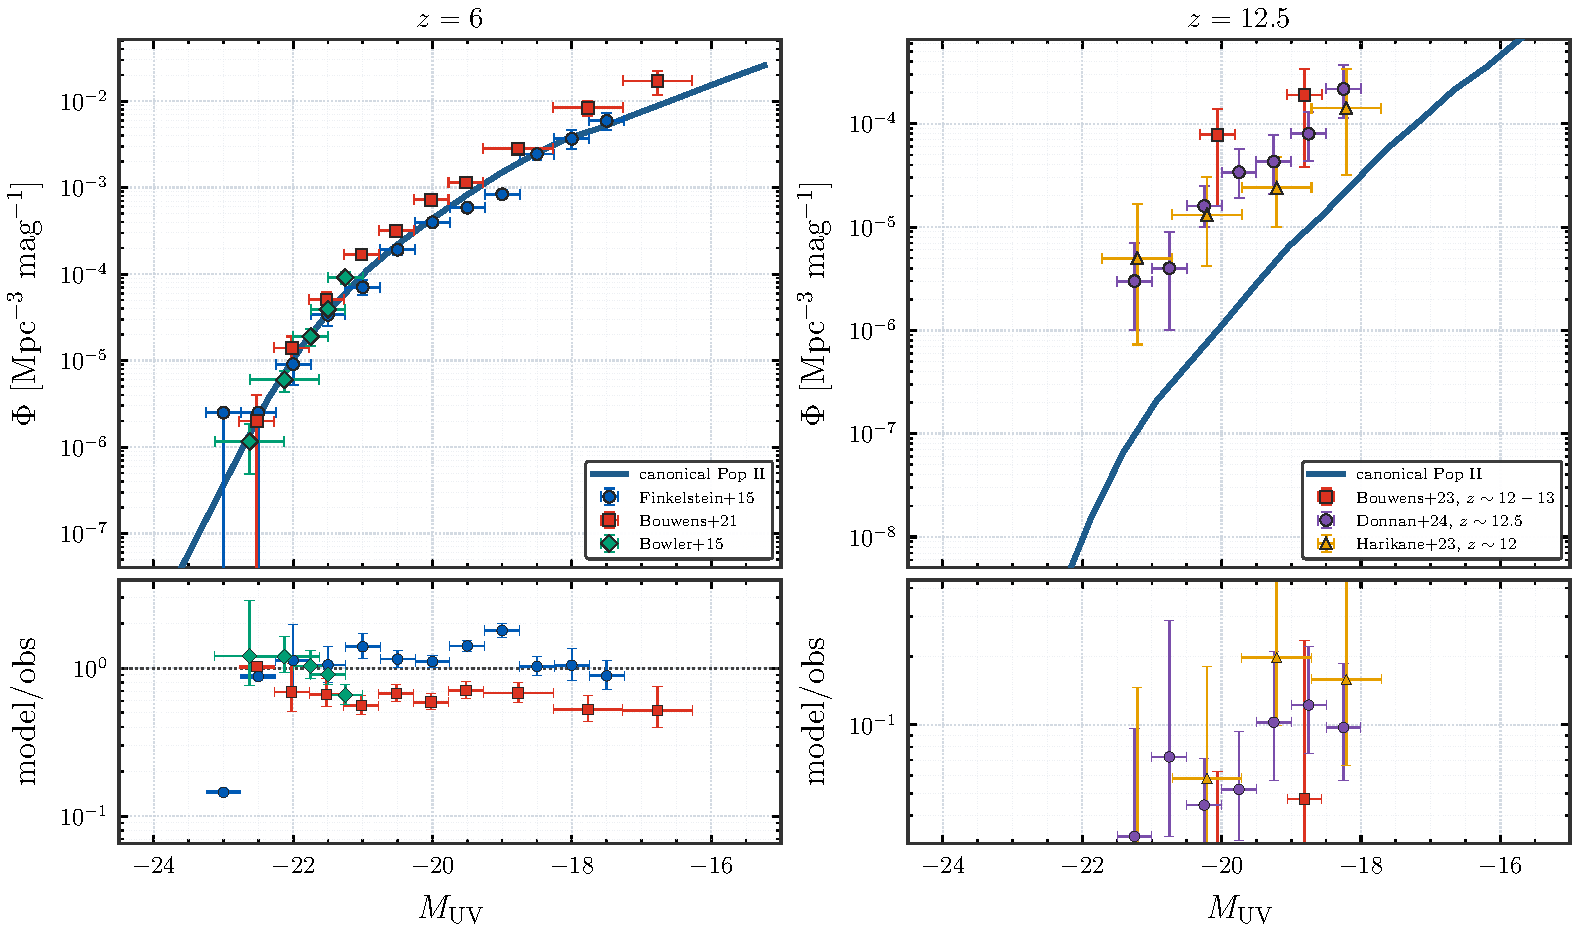
\includegraphics[width=\textwidth]{popii_uvlf_fit_check_z6_z12p5.pdf}
\caption{Population II UVLF baseline check at $z=6$ and $z=12.5$. The upper panels show the dust-attenuated canonical Population II UVLF against published UVLF measurements. The lower panels show the model/observation ratio evaluated at each observational magnitude bin. The $z=6$ data are from \citet{Finkelstein2015}, \citet{Bouwens2021} and \citet{Bowler2015}; the $z=12.5$ comparison uses \citet{Bouwens2023}, \citet{Donnan2024} and \citet{Harikane2023}. The result shows that the same Population II baseline that matches the $z=6$ scale remains low by roughly an order of magnitude at $z\simeq12.5$.}
\label{fig:popii-baseline-fit}
\end{figure*}

\begin{figure*}[tbp!]
\centering
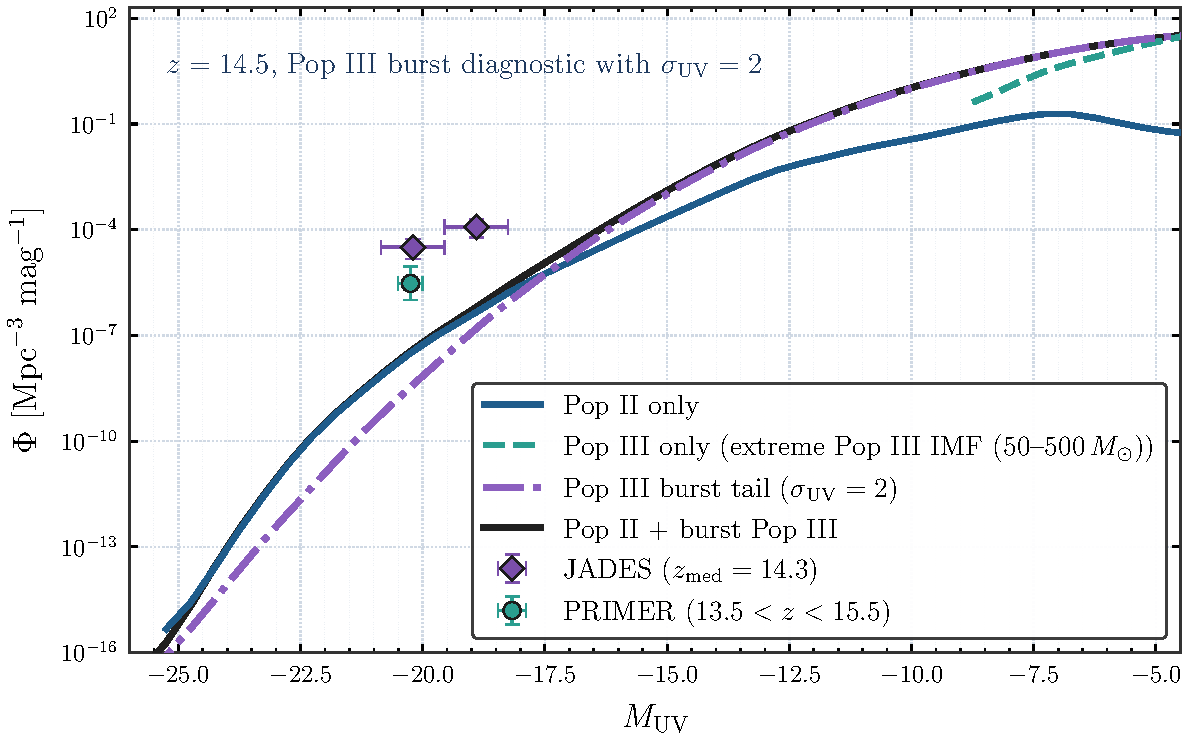
\includegraphics[width=\textwidth]{uvlf_z14p5_popii_popiii_components_slide.pdf}
\caption{UVLF component diagnostic at $z=14.5$. The Population II-only reference is compared with a Population III-only burst-tail contribution and their combined UVLF. The observed points are shown only as the current high-redshift reference scale for the diagnostic.}
\label{fig:uvlf-components}
\end{figure*}

\subsection{Population III cooling window}\label{subsec:cooling-window}

For zero external LW background, $J_{21}=0$, the ratio between the molecular-cooling floor and the Jeans mass, $M_{\rm min,III}/M_{\rm Jeans}$, is approximately 87.3, 17.3 and 6.55 at $z=10$, 20 and 30, respectively. The corresponding molecular-cooling floors are $5.91\times10^5$, $3.10\times10^5$ and $2.10\times10^5\,M_\odot$. These values remain below the atomic-cooling threshold, implying that a Population III minihalo window persists at high redshift in the absence of external LW feedback.

\subsection{Population III SFR density and LW feedback diagnostic}\label{subsec:popiii-sfrd-lw}

The current Population III channel produces an SFR-density history that is lower than the Population II baseline at low redshift but remains active across the high-redshift minihalo interval. A finite LW horizon proxy gives a first consistency check for feedback sensitivity: the no-external-LW and fixed-$J_{{\rm LW},21}=0.1$ tracks bracket the retained Population III contribution without yet closing the LW background back into the mass-routing calculation.

\begin{figure*}[tbp!]
\centering
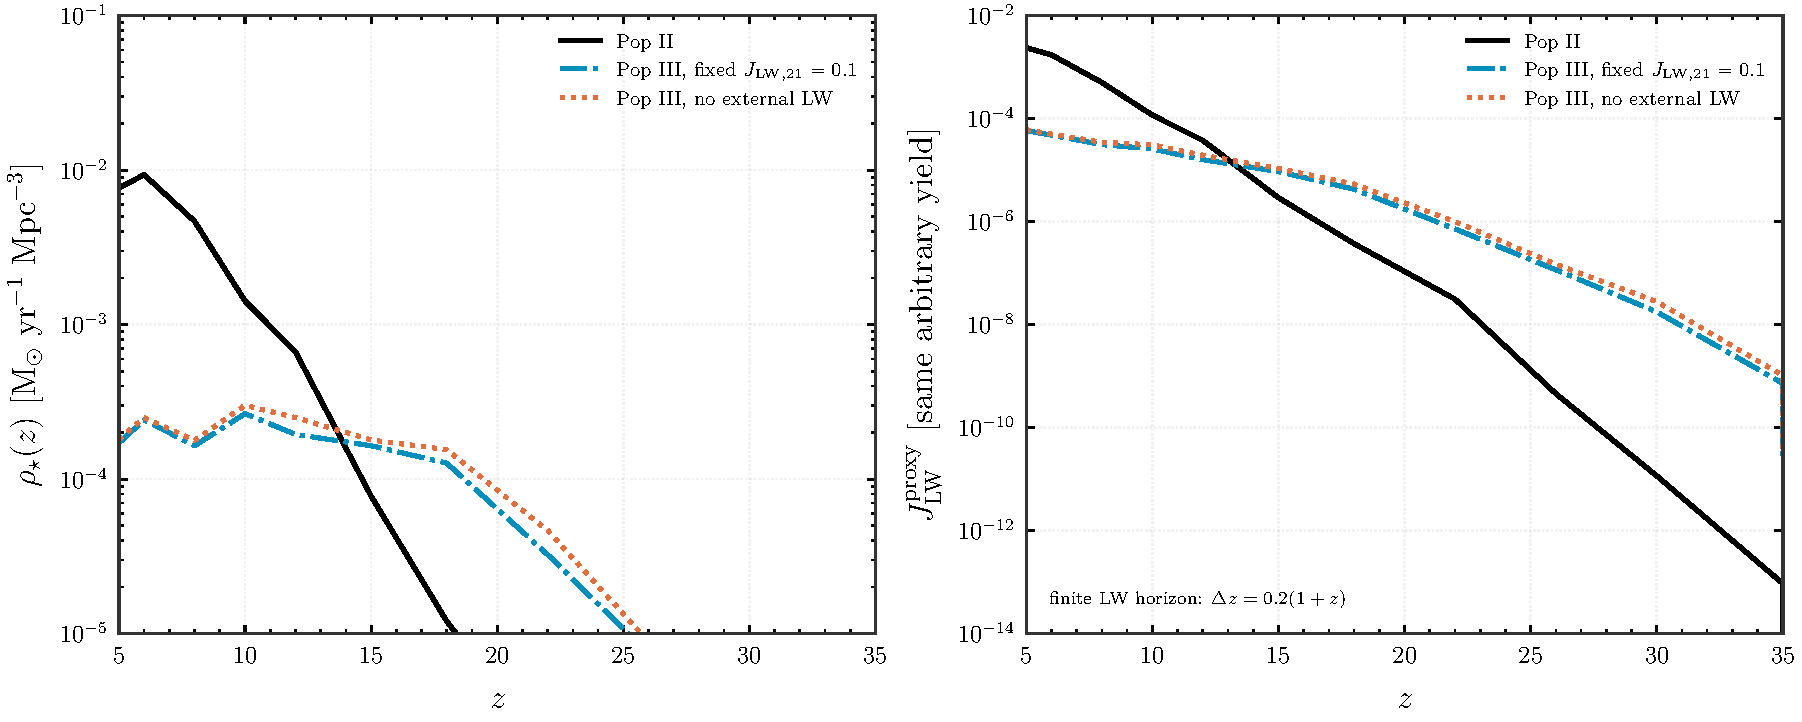
\includegraphics[width=\textwidth]{sfrd_lw_background_from_model_slide.pdf}
\caption{Population III SFR-density and LW-background proxy from the current model. The left panel compares the Population II and Population III SFR-density histories. The right panel shows a finite-horizon LW proxy used as a diagnostic for future feedback closure.}
\label{fig:sfrd-lw}
\end{figure*}

\subsection{Regulator metallicities against literature enrichment scales}\label{subsec:metallicity-result}

At $\log M_{\rm h}=8.5$, the \AuroraLF\ regulator gas metallicity differs from the polluted-IGM metallicity scale of \citet{Ventura2024} by roughly $-0.60$ to $+0.13$ dex. At $\log M_{\rm h}=9.5$, the offset changes from $-0.03$ dex at $z=7$ to $+3.62$ dex at $z=15$. The high-redshift, high-mass bin should be interpreted cautiously because the corresponding halo number density declines rapidly.

\section{Population III PISN diagnostic}\label{sec:pisn}

Once the Population III channel provides a volume-averaged SFR density, PISNe become an independent diagnostic of very massive metal-free stars. We adopt an extreme Population III IMF with Salpeter slope \citep{Salpeter1955} over $50\le M/M_\odot\le500$ and use $140\le M/M_\odot\le260$ as the PISN progenitor window \citep{HegerWoosley2002}. The number of PISN events per unit stellar mass formed is
\begin{equation}
  \eta_{\rm PISN}
  = \frac{\int_{140}^{260}\phi(M)\,\dd M}
  {\int_{50}^{500}M\phi(M)\,\dd M}
  =1.322\times10^{-3}\,M_\odot^{-1}.
\end{equation}
The corresponding intrinsic comoving PISN rate density is
\begin{equation}
  \dot n_{\rm PISN}(z)=\rho_{\rm SFR,III}(z)\,\eta_{\rm PISN}.
\end{equation}
This rate refers only to the adopted PISN mass window and should not be interpreted as the total Population III supernova rate.

\begin{figure*}[tbp!]
\centering
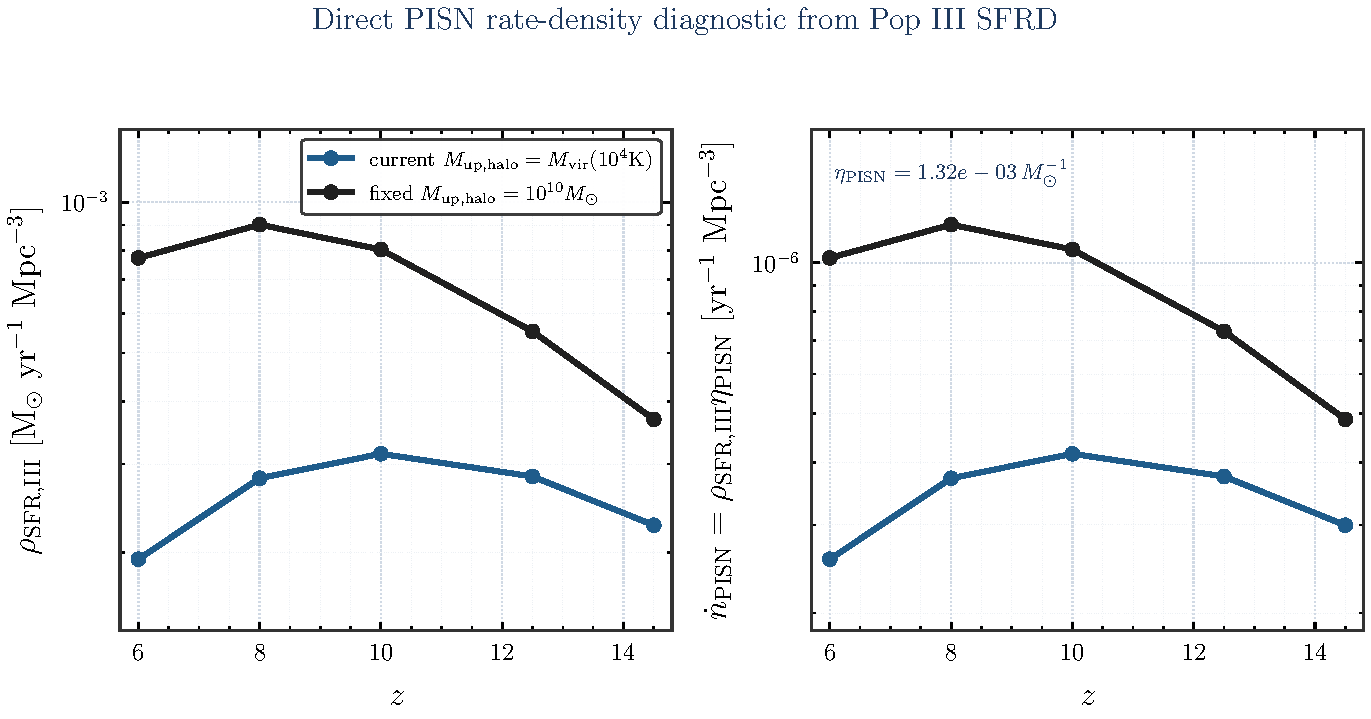
\includegraphics[width=0.86\textwidth]{popiii_mup_pisn_rate_from_sfr_two_panel.pdf}
\caption{Effect of the Population III upper halo-mass boundary on the PISN rate density. The blue curve shows the current atomic-cooling upper-bound model. The black curve shows a comparison model in which only the Population III upper halo mass is extended to $M_{\rm up}=10^{10}\,M_\odot$.}
\label{fig:pisn-rate}
\end{figure*}

\begin{table}[tbp]
\caption{PISN rate-density result for the two Population III upper-mass choices. The two rate columns are in ${\rm yr}^{-1}{\rm Mpc}^{-3}$.}
\label{tab:pisn-rates}
\centering
\scriptsize
\setlength{\tabcolsep}{2.8pt}
\begin{tabular}{cccc}
\toprule
$z$ & Current & $M_{\rm up}=10^{10}\,\Msun$ & Boost \\
\midrule
6.0  & $2.56\times10^{-7}$ & $1.02\times10^{-6}$ & 3.99 \\
8.0  & $3.72\times10^{-7}$ & $1.19\times10^{-6}$ & 3.21 \\
10.0 & $4.16\times10^{-7}$ & $1.06\times10^{-6}$ & 2.56 \\
12.5 & $3.75\times10^{-7}$ & $7.30\times10^{-7}$ & 1.95 \\
14.5 & $3.00\times10^{-7}$ & $4.87\times10^{-7}$ & 1.63 \\
\bottomrule
\end{tabular}
\end{table}

In the current atomic-cooling upper-bound model, $\dot n_{\rm PISN}$ at $z=6,8,10,12.5$ and 14.5 is $2.56\times10^{-7}$, $3.72\times10^{-7}$, $4.16\times10^{-7}$, $3.75\times10^{-7}$ and $3.00\times10^{-7}\,{\rm yr}^{-1}{\rm Mpc}^{-3}$, respectively. If only the Population III upper bound is extended to $M_{\rm up}=10^{10}\,M_\odot$, with all other parameters held fixed, the corresponding rates become $1.02\times10^{-6}$, $1.19\times10^{-6}$, $1.06\times10^{-6}$, $7.30\times10^{-7}$ and $4.87\times10^{-7}\,{\rm yr}^{-1}{\rm Mpc}^{-3}$. Extending the high-mass Population III interval therefore raises the PISN rate by about $2.6$--$4.0$ at $z=6$--10 and moves the result into the commonly discussed $10^{-6}\,{\rm yr}^{-1}{\rm Mpc}^{-3}$ range.

The enhancement is not caused by a change in $\eta_{\rm PISN}$, which is fixed by the IMF window. It is caused by the larger halo-mass interval contributing to the integrated Population III SFR density. The newly included interval $M_{\rm atom}\le M_{\rm h}<10^{10}\,M_\odot$ contributes 84.1\%, 82.1\%, 79.4\%, 72.2\% and 63.2\% of the added SFR density at $z=6,8,10,12.5$ and 14.5, respectively. This also shows that the bright end of the UVLF and the integrated PISN rate are not identical sensitivity tests: the former weights visible, luminous and short-timescale sources, whereas the latter directly integrates the Population III SFR density.

The present PISN result should be read as an intrinsic comoving rate-density diagnostic rather than a survey detection prediction. Existing long-timescale supernova searches mostly probe lower-redshift PISN-like events and do not directly exclude the $z>6$ rates considered here. A survey calculation requires
\begin{equation}
  \begin{split}
  N_{\rm det}={}&\int \dd z\,\dd\Omega\,
  \frac{\dot n_{\rm PISN}(z)}{1+z}
  \frac{\dd V}{\dd z\,\dd\Omega} \\
  &\times
  P_{\rm det}(z,{\rm light\ curve},{\rm cadence},m_{\rm lim}) .
  \end{split}
\end{equation}

\bibliographystyle{aasjournalv7}
\bibliography{references}

\end{document}
